\section*{Part B: Temperature Sensors}
\addcontentsline{toc}{section}{Part B: Temperature Sensors}

\paragraph{Task 3 a) Bias-related sensitivity of the bridge.}
With $V_B$ at the top, the left arm is $R_1$ (top)\,$+$\,$R_3$ (bottom) and the right arm is
$R_2$\,$+$\,$R_4$; the output is $V_o=V_A-V_C$ across the two mid-nodes. The figure pairs
opposite-TCR resistors in adjacent arms ($R_1,R_4$ negative; $R_2,R_3$ positive), which is the
fully-active configuration. Writing $R_n=R(1+\alpha_{\mathrm{neg}}\Delta T)$ and
$R_p=R(1+\alpha_{\mathrm{pos}}\Delta T)$,
\[
V_o=V_B\!\left[\frac{R_3}{R_1+R_3}-\frac{R_4}{R_2+R_4}\right]
   =V_B\,\frac{(\alpha_{\mathrm{pos}}-\alpha_{\mathrm{neg}})\,\Delta T}{2+(\alpha_{\mathrm{pos}}+\alpha_{\mathrm{neg}})\,\Delta T}.
\]
The bias-related sensitivity is the output per unit bias per kelvin, evaluated at balance
($\Delta T\!\to\!0$):
\[
S_{\mathrm{bias}}=\frac{1}{V_B}\frac{\partial V_o}{\partial T}\bigg|_{0}
=\frac{\alpha_{\mathrm{pos}}-\alpha_{\mathrm{neg}}}{2}
=\frac{5\times10^{-4}-(-3\times10^{-4})}{2}
=\mathbf{4\times10^{-4}\ \si{\per\kelvin}}\;(=\SI{0.4}{\milli\volt\per\volt\per\kelvin}).
\]

\paragraph{Task 3 b) SNR vs.\ temperature.}
\textbf{Signal:} the output grows essentially linearly with $\Delta T$,
$V_o\approx V_B(\alpha_{\mathrm{pos}}-\alpha_{\mathrm{neg}})\Delta T/2$, and is \emph{zero} at the
balance point $T_0$. \textbf{Noise:} the dominant term is the thermal noise of the bridge's output
resistance, $u_n=\sqrt{4k_BT\,R_{\mathrm{out}}\,\mathrm{ENBW}}$, which depends only weakly on
temperature. For the symmetric case $\alpha_{\mathrm{neg}}=-\alpha_{\mathrm{pos}}$ the two TCRs
cancel in $R_{\mathrm{out}}$, so $R_{\mathrm{out}}\approx R$ stays constant and the only temperature
dependence of the noise is the slow $\sqrt{T}$. Hence
\[
\mathrm{SNR}=\frac{V_o}{u_n}\propto\frac{\Delta T}{\sqrt{T}} .
\]
The SNR is zero at $T_0$ and \emph{increases monotonically} as the temperature moves away from
balance, because the numerator climbs linearly while the noise rises only as $\sqrt{T}$.

\textbf{Additional task: exact SNR.} Using the exact $V_o(T)$,
$R_{\mathrm{out}}=2R_nR_p/(R_n+R_p)$ and $u_n=\sqrt{4k_BT\,R_{\mathrm{out}}\,\mathrm{ENBW}}$ with
$V_B=\SI{5}{\volt}$, $R=\SI{1}{\kilo\ohm}$, $\mathrm{ENBW}=\SI{1}{\kilo\hertz}$ and the part-a)
$\alpha$-values gives Fig.~\ref{fig:snr}. The curve rises from $-\infty$ at the \SI{300}{\kelvin}
balance point to about \SI{122}{dB} at \SI{400}{\kelvin}.

\begin{figure}[H]
\centering
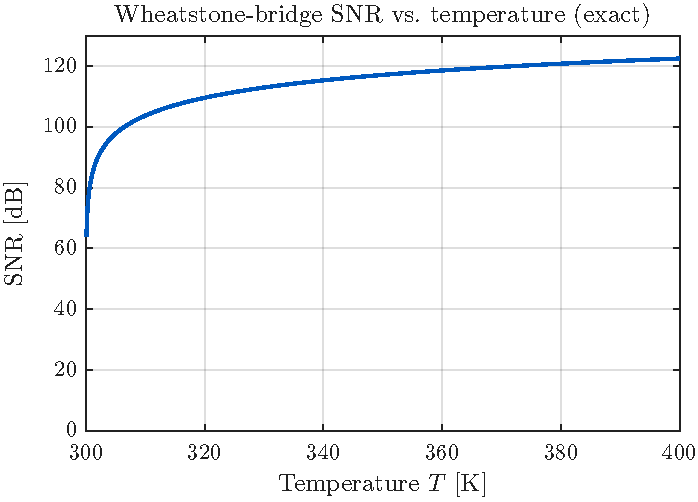
\includegraphics[width=0.62\textwidth]{figures/q3b_snr.pdf}
\caption{Exact Wheatstone-bridge SNR over \SIrange{300}{400}{\kelvin}. The output (and hence the
SNR) vanishes at the \SI{300}{\kelvin} balance point and grows steadily as $|\Delta T|$ increases.}
\label{fig:snr}
\end{figure}

\paragraph{Task 3 c) Measures for sufficient SNR (Additional).}
The problem is the dead zone near $T_0$, where $V_o\to0$. Practical fixes:
\begin{itemize}[nosep,leftmargin=1.4em]
\item \textbf{Offset the bridge} (unbalance it deliberately, e.g.\ trim one arm) so $V_o\neq0$ at the
low end. \emph{$+$} removes the dead zone; \emph{$-$} costs dynamic range and adds offset drift.
\item \textbf{Raise the bias $V_B$:} $\mathrm{SNR}\propto V_B$ while thermal noise is independent of
it. \emph{$+$} direct gain; \emph{$-$} power $\propto V_B^2$ $\Rightarrow$ self-heating error.
\item \textbf{Reduce ENBW / average longer:} noise $\propto\sqrt{\mathrm{ENBW}}$. \emph{$+$} cheap SNR;
\emph{$-$} slower measurement (energy $\times$ time trade-off).
\item \textbf{Higher-TCR materials} (larger $\alpha_{\mathrm{pos}}-\alpha_{\mathrm{neg}}$).
\emph{$+$} more signal; \emph{$-$} worse nonlinearity, needs polynomial correction.
\end{itemize}
